\section{Face alignment}
Facial alignment is a normalization technique often used to improve accuracy of face recognition algorithms which include deep learning methods that we used. The goal of a face alignment algorithm is to transform a dataset with face images so that each face should be centered in the image, rotated such that the eyes lie on a horizontal line and be scaled to a fixed size.
The process of face alignment is structured on two steps: the first one represents the detection of facial landmarks on the input image and the second one is the appliance of an affine transformation so that in the output image, the detected facial landmarks are at the same position every time.
\subsection{Face landmarks detection}
\begin{figure}[h]
	\begin{center}
		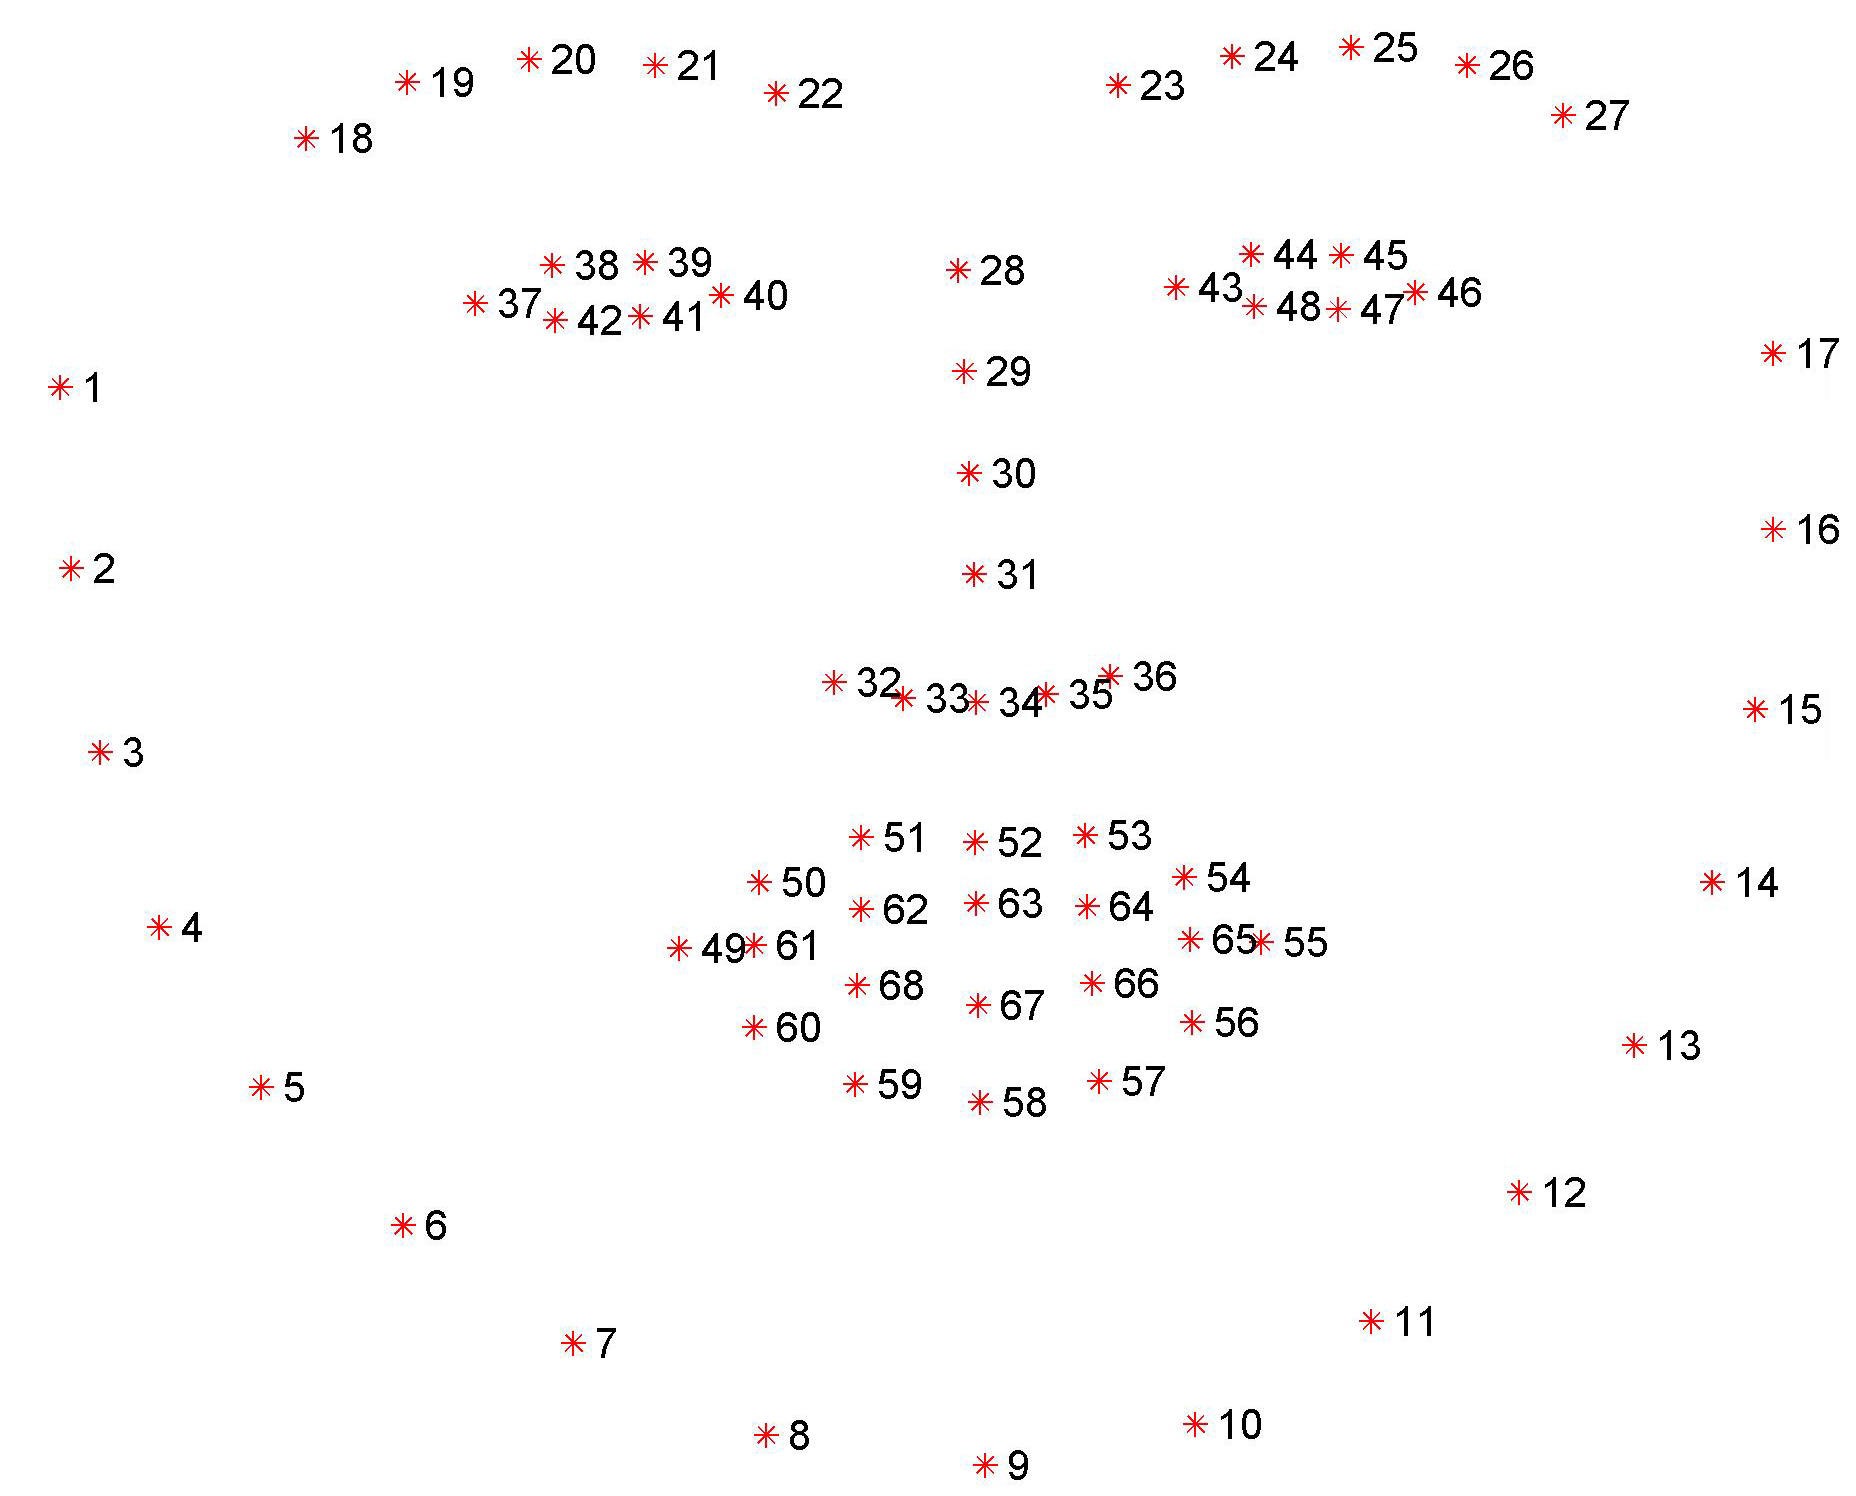
\includegraphics[width=15cm]{facial_landmarks}
		\caption[Facial landmarks visualisation]{Visual representation of the 68 points representing face landmarks}
	\end{center}
\end{figure}
We will broadly present the method of determining the facial landmark in an image as suggested in \cite{kazemi2014one}. The main idea is to create a cascade of regressors where each one will improve the predicted landmarks vector based on the result of the previous one. Therefore, following the explanation in \cite{kazemi2014one}, letting $x_{i} \in \rm I\!R^{2}$ represent the $x,y - $ coordinates of the $i$th facial landmark and using $S = (x_{1}^{T}, x_{2}^{T}, ..., x_{p}^{T})^{T} \in \rm I\!R^{2p}$ as notation for the coordinates of all $p$ facial landmarks also referred to as shape, we can denote by $\hat{S}^{(t)}$ the estimation of the landmarks at step $t$. Each regressor $r(\cdot, \cdot)$ in the cascade predicts an update of the estimated shape from the input image and the previous estimation following the formula
\begin{align}
	\hat{S}^{(t+1)} = \hat{S}^{(t)} + r(I, \hat{S}^{(t)})
\end{align}
Kazemi and Sulivan state in \cite{kazemi2014one} that the key aspect of the cascade is that the regressor $r_{t}$ makes its prediction based on features computed from image $I$ and indexed relative to the current shape estimation $\hat{S}^{(t)}$. This introduce some form of geometric variance in the process. The method used to learn the regressors is gradient boosting with regression trees as the base learner for the pseudo-residuals. One thing to note is that after learning one regressor, it's output becomes the training data for the following one. The exact algorithm, as well as the specifics of the regression trees are described in details in section 2 of \cite{kazemi2014one}.

\subsection{Face affine transformation}
Once we detect the facial landmarks, the next step in the face alignment process is appliance of an affine transformation. This way, the landmarks are brought to the expected positions in the image. So, having the actual and the expected position of the face landmarks we compute $T$, the $2\times3$ matrix of an affine transformation so that:
\begin{align}
	\begin{bmatrix}
	x_{i}'\\
	y_{i}'
	\end{bmatrix}
	=
	T \cdot
	\begin{bmatrix}
	x_{i}\\
	y_{i}\\
	1
	\end{bmatrix}
\end{align}
where $x_{i}', y_{i}'$ and $x_{i}, y_{i}$ are the expected and the actual coordinates of the $i$th facial landmark. Here we note that not all landmarks must be aligned, this depends on the use case. Only a few like inner eyes and bottom lips or outer eyes and nose landmarks are sometimes sufficient.

Having known the matrix of the affine transform, we then apply it to the source image:
\begin{align}
	dst(x, y) = src(T_{1,1}x + T_{1,2}y + T_{1,3}, T_{2,1}x + T_{2,2}y + T_{2,3})
\end{align} where $dst$ is the resulting image, $src$ is the source image and $T$ is matrix specified as the affine transform. 